\section{Implementering}
\label{sec:implementering}
\textit{Enda mer \textbf{hvordan} kommer her. Nå er vi på detaljnivå med detaljerte kretsskjema og dokumentasjon av algoritmer og kode. Større mengder kildekode er ikke aktuelt å ta med, men kortere snutter for å beskrive spesielle løsninger kan tas med. Resten av kildekoden legges ved som vedlegg. \\
\\
Detaljer puttes i vedlegg.}

Overordnet består systemet av to delsystemer. Det ene delsystemet detekterer og sporer fugleaktivitet med et varmekamera, og det andre delsystemet henter inn værdata. Begge disse systemene sender data til en Raspberry Pi 4, som så prosesserer dataen og sender det videre til en database, før det blir framstilt på en nettside. 

\begin{figure}[H]
    \centering
    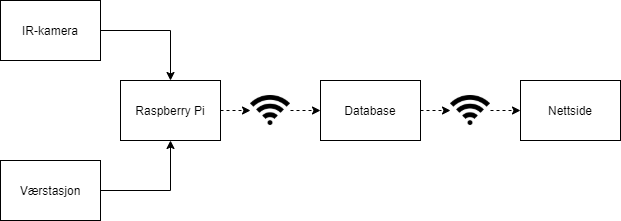
\includegraphics[width=0.8\textwidth]{implementering/implementering.png}
    \caption{Overordnet flytskjema for hele systemet.}
    \label{fig:implementasjon}
\end{figure}


\subsection{Prossesseringsenhet}\todo{Burde endres til prosessor eller noe sånt}

Til databehandling brukes en Raspberry Pi 4. Dette er en liten PC på ett enkelt kretskort, men som tilbyr nok minne og prosesseringskraft til dette systemets formål. Pi-en utfører all bildebehandling samt prosessering av værdata og trådløs overføring av data til databasen. I dette systemet brukes en Raspberry Pi modell 4B, med 4GB RAM og en 64-bits prosessor.

\begin{figure}[H]
    \centering
    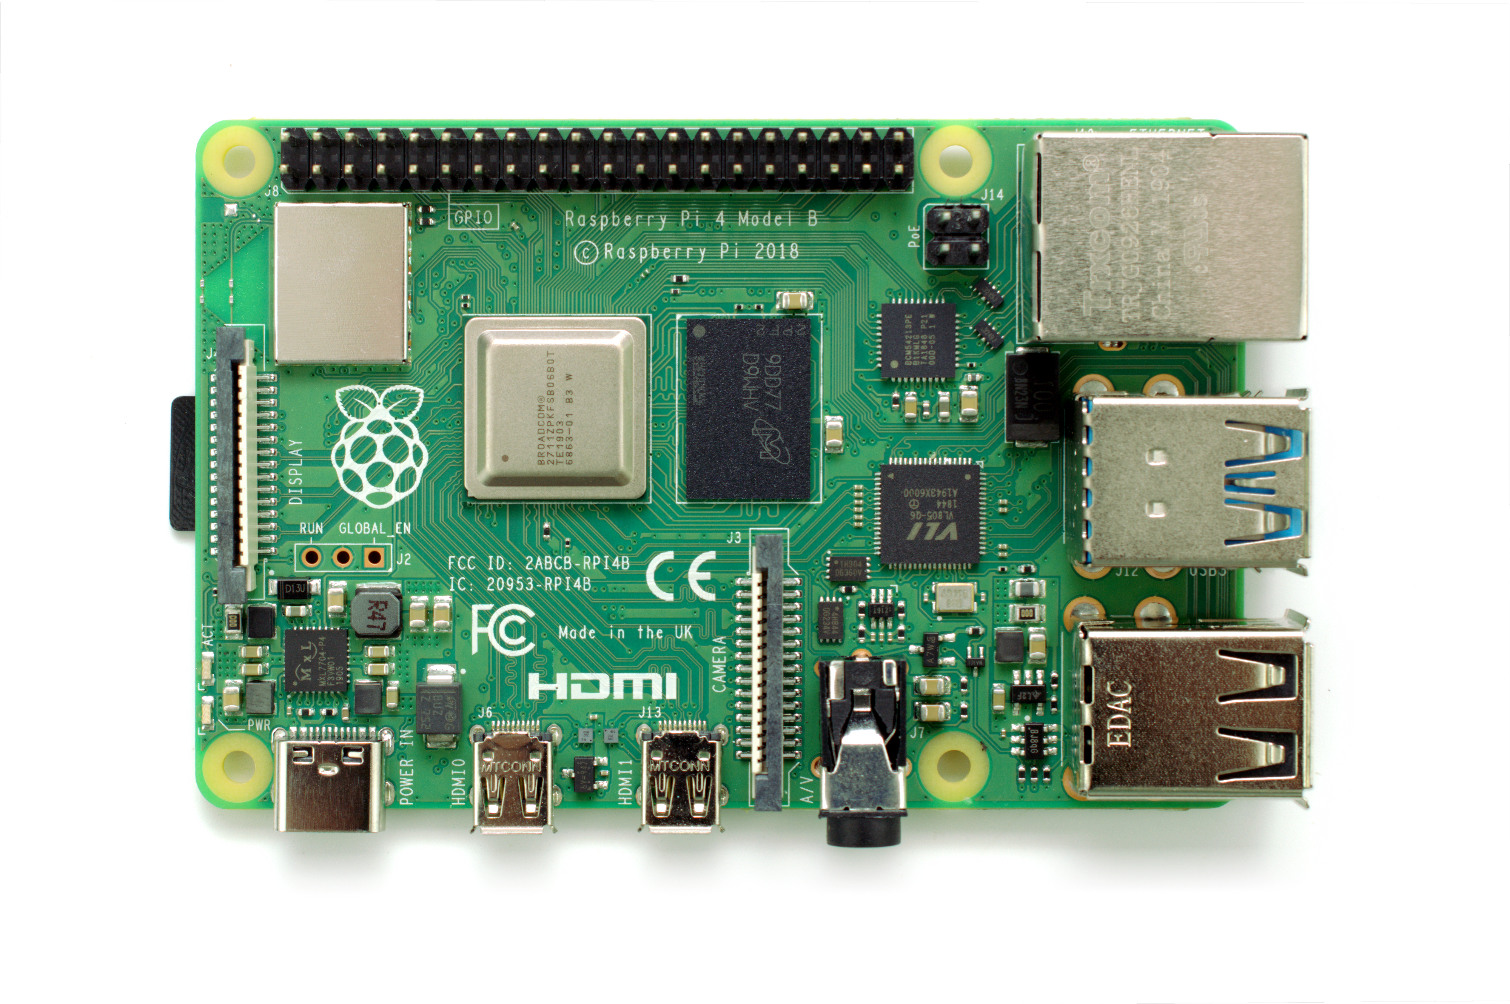
\includegraphics[width=0.5\textwidth]{implementering/pi4.png}
    \caption{Raspberry Pi 4.}
    \label{fig:pi}
\end{figure}

%en referanse til Pi4? datablad elns?

\subsection{Kamera}

Det infrarøde kameraet som benyttes er et FLIR (Forward-Looking InfraRed) C3-kamera. C3 er
håndholdt, men kan også brukes koblet til en datamaskin, her en Raspberry Pi. Kameraet har en IR-sensor med synsvinkel på $41\degree \text{x} 31\degree$, bilderate på 9 Hz, og kan detektere temperaturforskjeller på under $0.1\degree$C. Kameraet vil kontinuerlig ta bilder med en valgbar frekvens, som optimaliseres for å gi best mulig deteksjon. Samtidig må denne begrenses slik at bildebehandlingen ikke havner bakpå. Bildene overføres til Pi-en via USB-kabel.


\begin{figure}[H]
    \centering
    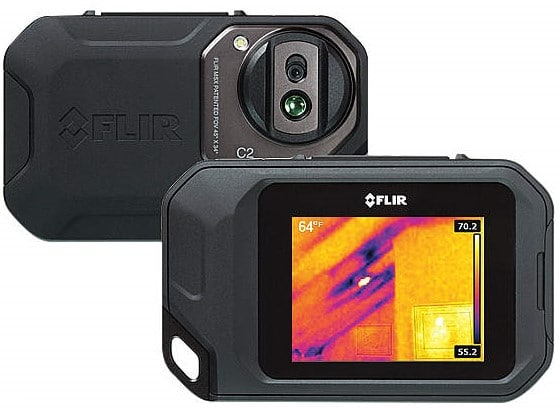
\includegraphics[width=0.5\textwidth]{implementering/c3.png}
    \caption{FLIR C3.}
    \label{fig:c3}
\end{figure}


\subsection{OpenCV}

OpenCV er et bibliotek som gir utviklere rask og enkel tilgang til avanserte algoritmer innen maskinlæring og datasyn. Disse kan brukes til å filtrere bilder, detektere objekter og utføre tracking fra bilde til bilde. \todo{fyll på mer info}

\subsection{Programvare} \todo{fiks figurer}

Programmet som kjøres på Pi-en er skrevet i Python. Hovedflyten til programmet er vist i \autoref{fig:hovedprogram}. Ved oppstart kjører programmet gjennom en startprosedyre før det går inn i en loop med sykliske hendelser. Oppsettfasen initialiserer blant annet logging, telemetri, sensorer og bildeprosessering, slik at disse tingene er satt i gang og testet og dermed klar til bruk. Deretter forsetter programmet å kjøre gjennom en rekke sykliske hendelser for bildegjennkjenning, sensorer samt telemetri og logging. Mer om dette etterhvert.\todo{fyll inn noe om error-biten}

\begin{figure}[H]
    \centering
    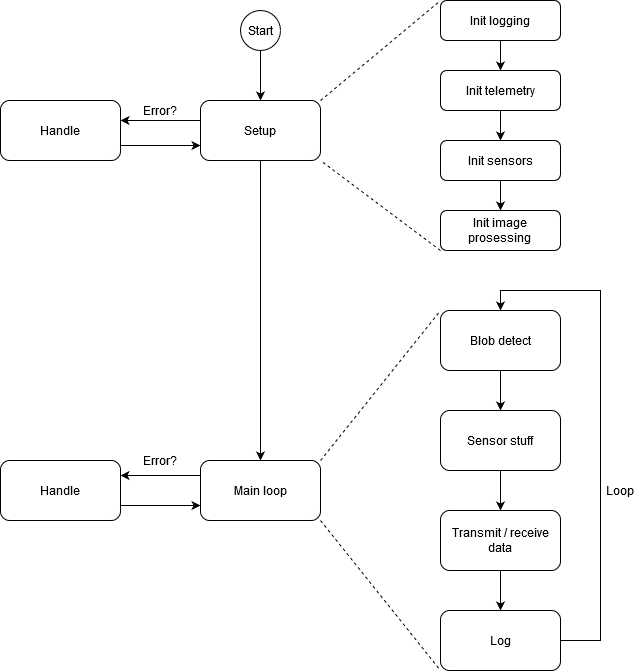
\includegraphics[width=0.8\textwidth]{implementering/hovedprogram.png}
    \caption{Flytskjema for det overordnede systemet.}
    \label{fig:hovedprogram}
\end{figure}

\subsubsection{Bildeprosessering}

En datamaskin har ingen måte å kunne kjenne igjen en fugl fra et bilde. Dette er et eksempel på en veldig komplisert type problemstilling ingeniører har jobbet med i årevis. OpenCV tilbyr en god del verktøy, som implementerte algoritmer for filtrering, som hjelper oss til å kunne løse dette problemet. 

Flyten for bildeprosessesseringen er illustrert i \autoref{fig:bildeprosessering}.  \todo{skriv mer om opencv med kilde?}

\begin{figure}[H]
    \centering
    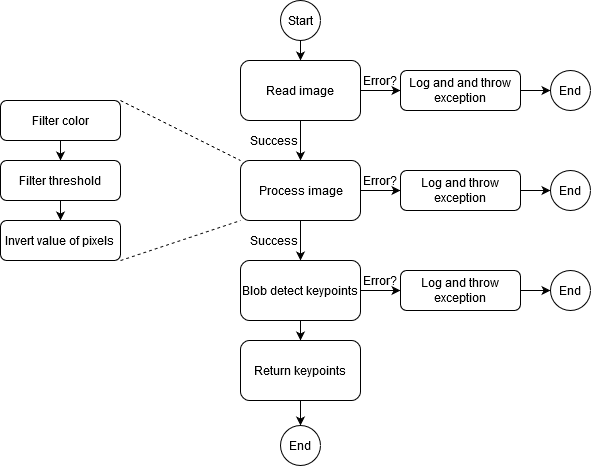
\includegraphics[width=0.8\textwidth]{implementering/bildeprosessering.png}
    \caption{Caption}
    \label{fig:bildeprosessering}
\end{figure} \todo{return? ikke end? Burde være på norsk?}

OpenCV  har en innbygd funksjon for å lese inn videostrømmer slik at IR-kameraet kan benyttes som om det var et vanlig webkamera. Det er altså forholdsvis enkelt å få en bildestrøm inn til Pi-en. Dermed blir problemet for koden i hovedsak hvordan denne strømmen av bilder skal filtreres og analyseres for å kunne detektere blobs og hvordan disse blobbene kan spores fra bilde til bilde. En blob, eller klump på norsk, er en samling av piksler som skiller seg fra bakgrunnen. Et eksempel på dette er en svart fugl mot en blå himmel. Det er ganske enkelt for et menneske å forstå dette, og kunne se hvor denne blobben befinner seg. Oppgaven blir mer krevende når en datamaskin skal gjøre det. 

For å lettere og mer presist kunne analysere blobs må bildene filtreres.


Videre kan innebygde funksjoner i OpenCV som  detekterer blobs i bilder brukes. OpenCV gir flere metoder for å utføre dette, men i første omgang velges simple blob detector. Denne tar inn et bilde og parametere \todo{finne ut hva den faktisk tar inn og hva keypoints faktisk inneholder} og returnerer en liste over keypoints, altså en liste over koordinatene til slike blobs.
\todo{legge inn kode}


\subsubsection{Tracking}
\label{subsubsec:tracking}
For å unngå at programmet teller samme fugl flere ganger, selv om fuglen er i videostrømmen i flere bilder etter hverandre, brukes tracking. Måten trackingen fungerer er at den gis koordinater til et område på skjermen der det finnes et objekt, som her vil være en fugl. Dette objektet vil den kjenne igjen når neste bilde kommer, og den vil klare å følge objektet gjennom videostrømmen.
Siden det kan være flere fugler i bildet samtidig trengs det å kunne tracke alle sammen. Dette gjøres ved å lage et multi-tracker objekt som samler flere trackere som følger forskjellige fugler. Ved bruk av flere trackere er det viktig at samme fugl ikke trackes med flere trackere slik at en fugl blir talt flere ganger. Ved å ikke opprette trackere der det allerede finnes en tracker fra før av unngås dette. 

Når en fugl skal trackes behøves koordinatene til fuglen i bildet. Dette fås fra blob-detection koden. Blob-detection koden returnerer et keypoint, som inneholder senter og radius til bloben. Trackerfunksjonen tar inn en firkantet boks som må omslutte bloben helt. Derfor er det behov for en funksjon som kan gjøre om keypoints til bokser. Dette er vist i \autoref{code:keypointsToBoxes}. Funksjonen returnere en liste som inneholder all info om boksene som trengs til trackingen.
\begin{code}
\begin{minted}[mathescape,
               linenos,
               numbersep=5pt,
               gobble=2,
               frame=lines,
               framesep=2mm]{python}
    import cv2
    
    def KeypointsToBoxes(keypoints):
    boxes = []
    for keypoint in keypoints:
        point = keypoint.pt
        size = int(keypoint.size)
        box = (int(point[0])- (size/2),int(point[1]) - (size/2),size,size)
        boxes.append(box)
    return boxes
\end{minted}
\caption{Hvordan keypoints fra blob-detection blir gjort om til bokser som kan brukes i tracking.}
\label{code:keypointsToBoxes}
\end{code}

Når alle keypoints er gjort om til bokser, må det finnes ut hvilket blobber som allerede trackes, Det kan gjøres ved å sjekke om midten av noen av blobbene ligger innenfor boksen til en blob som allerede trackes. Hvis den gjør det må ikke blobben trackes på nytt. I \autoref{code:removeTrackedBlobs} vises det hvordan dette kan gjøres.

\begin{code}
\begin{minted}[mathescape,
               linenos,
               numbersep=5pt,
               gobble=2,
               frame=lines,
               framesep=2mm]{python}
    def removeTrackedBlobs(keypoints, boxes):
        newKeypoints = []
        diff = []
        try:
            for points in keypoints:
                x = points.pt[0]
                y = points.pt[1]
                for box in boxes:
                    xb,yb,wb,hb = box
                    if xb<x and x<xb+wb and yb<y and     y<yb+hb:
                        diff.append(points)
            for point in keypoints:
                if point not in diff:
                    newKeypoints.append(point)
        except:
            pass
        return newKeypoints
\end{minted}
\caption{Her vises det hvordan det sjekkes om blobber er nye i bildet eller om de trackes fra et tidligere bilde.}
\label{code:removeTrackedBlobs}
\end{code}

OpenCV i Python har flere funksjoner som hjelper til med denne trackinga, og har flere forskjellige metoder for tracking, som varierer i nøyaktighet og tidsbruk.

For å opprette en tracker for en blob kalles funksjonen createTrackerByName som ligger i trackerFunc.py. Denne funksjonen mottar hvilken type tracker som skal brukes. I tillegg må man initialisere trackeren ved å si hvilket bilde bloben er i koordinater til en boks som skal omslutte bloben. Siden det kan være flere fugler i et bilde er det nødvendig å kunne lage flere trackere, og lagre disse sammen.

OpenCV har en multitrackerklasse, men denne er ikke tilfredsstillende, da det ikke kan slettes trackere fra et multitracker-objekt. Derfor er en ny klasse implementert i python med de ønskede egenskapene. En del av implementeringen av denne klassen kan sees i \autoref{code:newTracker}. Klassen består av to lister. Listen trackers består av enkle trackere, og listen trackerFail består av tall. Disse tallene forteller i hvor mange bilder etter hverandre trackeren har mislyktes med å følge en blob. Når blob-detection algoritmen har kjørt legges alle nye blobs til med medlemsfunksjonen add.
\begin{code}
\begin{minted}[mathescape,
               linenos,
               numbersep=5pt,
               gobble=2,
               frame=lines,
               framesep=2mm]{python}
    class NewTracker():                     
        def __init__(self):
            self.trackers = []             
            self.trackerFail = []
    
        def add(self, trackerObj):          
            self.trackers.append(trackerObj)
            self.trackerFail.append(0)
\end{minted}
\caption{En del av implementeringen av multitrackeren.}
\label{code:newTracker}
\end{code}
I tillegg har klassen medlemsfunksjonene pop og update. Funksjonen pop fjerner trackere, og update oppdaterer alle trackere. I tillegg til å oppdatere trackerene vil update-funksjonen inkrementere listeelementene i trackerFail som hører til trackere som mislyktes med sporingen sin. Dersom trackeren klarte å følge bloben blir tilhørende trackerFail-element satt til 0. Alle trackere som ikke har detektert bloben sin i 5 bilder på rad vil fjernes fra multitrackeren. Funksjonen update returnerer også en liste med koordinatene til alle trakcerene.


\subsubsection{Telemetri}
\label{subsubsec:telemetri}

Kommunikasjon mellom Pi-en og nettsiden går via en Firebase-database, levert av Google. Denne kommunikasjonen foregår over Wi-Fi. Dataene Pi-en samler inn blir sendt til databasen som dictionaries og lagret der på et NoSQL-format. En NoSQL-database er ikke så streng med struktur, så den takler bedre endringer i strukturen til dataene. Firebase har laget gode Python-bibliotek som gjør overføring fra Pi-en enkelt. Måten dette fungerer på blir abstrahert bort av ferdigutviklet software, som ligger i firebase\_admin biblioteket. All data i databasen har en nøkkel som er en timestamp som angir når det ble lastet opp i databasen. Når data blir hentet fra databasen kan det sorteres etter nøklene eller de forskjellige dataene som ligger der.

\subsubsection{Logging}
I programmet er det ikke alltid at ting fungerer som det skal. Derfor er det svært nyttig å ha en logging-fil der all viktig informasjon om det programmet har gjort ligger. De operasjonene programmet gjør vellykket, og som er viktig informasjon som kan brukes senere, i tillegg til hva programmet ikke har fått til er informasjon som blir lagt til i logging-fila. Alt som blir lagt til i logging-fila blir også merket med hvor viktig informasjonen er, for eksempel INFO eller CRITICAL. 

\subsection{Værstasjon}

Værstasjonen vil måle temperatur, trykk og fuktighet i lufta, i tillegg til vindhastighet, vindretning og nedbørsmengde. All dataen sendes via et kretskort til Raspberry Pi-en, som prosesserer dataen og sender det videre til databasen, så informasjonen blir tilgjengelig i nettsiden. \autoref{fig:kretsskjema_pi} viser oppkoblingen til Raspberry Pi-en.

\begin{figure}[H]
    \centering
    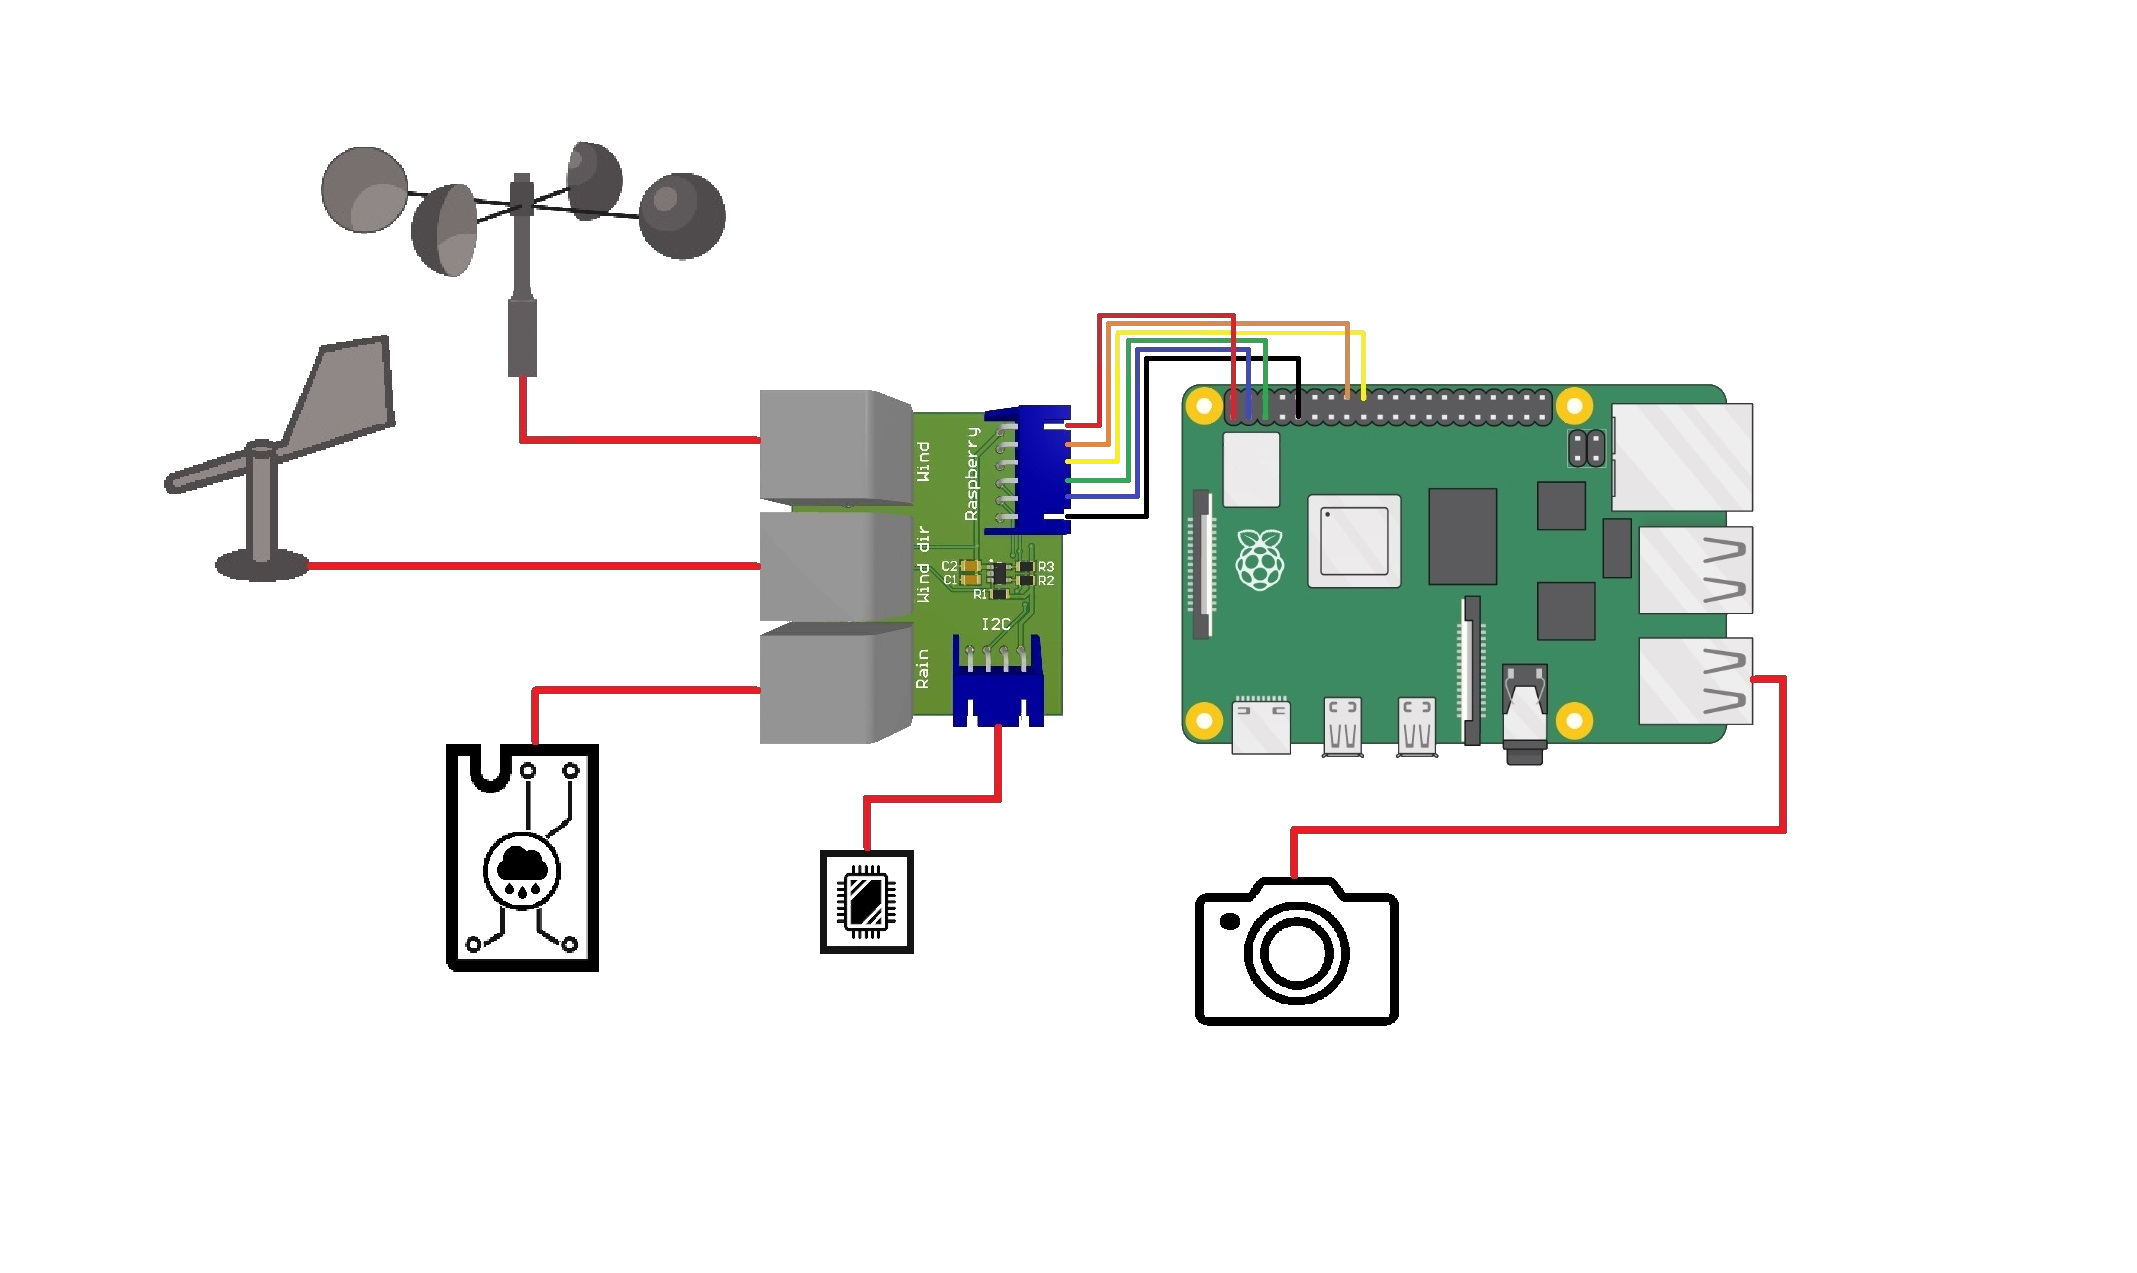
\includegraphics[width=\textwidth]{implementering/kretsskjema_pi.png}
    \caption{Figuren viser oppkoblingen av Raspberry Pi, kretskort, og sensorer. Mer spesifikt her om hva som er koblet til hvilke porter og noder?}
    \label{fig:kretsskjema_pi}
\end{figure}

\subsubsection{Trykk, temperatur, luftfuktighet}

All luftdataen hentes fra en BME280-sensor fra Bosch, som kan måle både temperatur, trykk og fuktighet i lufta. Kommunikasjonen mellom sensoren og Raspberry Pi-en foregår over en I2C-protokoll, en synkron, seriell bussprotokoll. Figur x og x under viser henholdsvis kretstegning og 3d-modell av luftsensoren.

\begin{figure}[H]
    \centering
    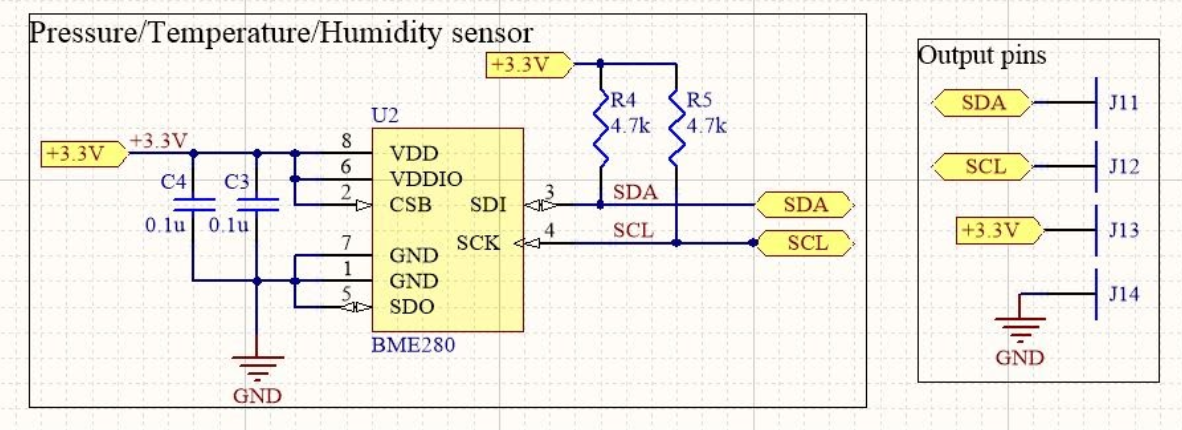
\includegraphics[width=0.9\textwidth]{implementering/luftsensor_krets.png}
    \caption{Kretsskjema for luftsensoren.}
    \label{fig:luftsensor_krets-}
\end{figure}

\begin{figure}[H]
    \centering
    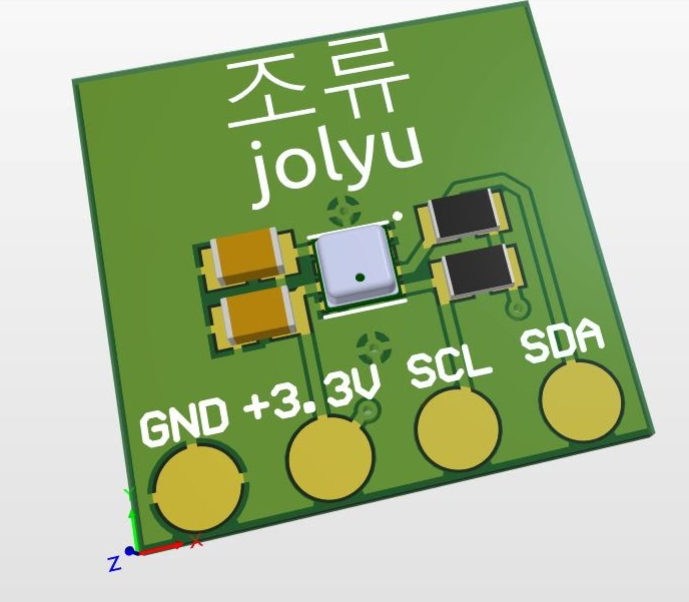
\includegraphics[width=0.5\textwidth]{implementering/luftsensor_3d.png}
    \caption{3D-modell av luftsensoren.}
    \label{fig:luftsensor_3d}
\end{figure}

%https://ae-bst.resource.bosch.com/media/_tech/media/datasheets/BST-BME280-DS002.pdf

\subsubsection{Anemometer}

Anemometeret som brukes måler vindhastigheten ved å lukke en bryter når en magnet beveger seg forbi bryteren. Måleren bruker en reed-bryter, en bryter som lukkes når det er et magnetfelt tilstede. Denne bryteren lukkes én gang for hver omdreining. Ved å telle antall ganger bryteren lukkes per tidsenhet kan rotasjonshastigheten til vindmåleren beregnes. Dette kan igjen brukes til å regne ut vindhastigheten. I følge databladet vil bryteren lukkes én gang i sekundet ved en vindhastighet på 2.4 km/h ~ 0.67 m/s.


\begin{figure}[H]
    \centering
    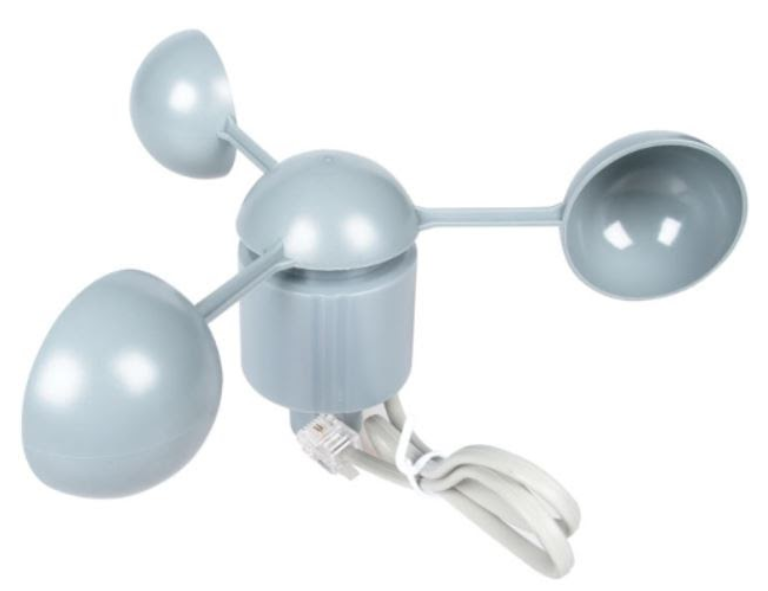
\includegraphics[width=0.5\textwidth]{implementering/anemometer.png}
    \caption{Anemometeret,}
    \label{fig:anemometer}
\end{figure}


%https://www.argentdata.com/files/80422_datasheet.pdf

\subsubsection{Vindretning}

Retningsmåleren består av 8 reed-brytere plassert i en sirkel, slik at det er $45\degree$ mellom hver bryter. En magnet vil rette seg mot vinden, og vil lukke en eller to reed-brytere om gangen. Dett resulterer i totalt 16 posisjonskombinasjoner, og dermed en nøyaktighet på $\pm 11.25\degree$. De 16 ulike kombinasjonene vil koble signalpinen til 16 ulike motstandsverdier, som kan leses som et analogt signal for å finne retningen ved hjelp av en spenningsdeler.


\begin{figure}[H]
    \centering
    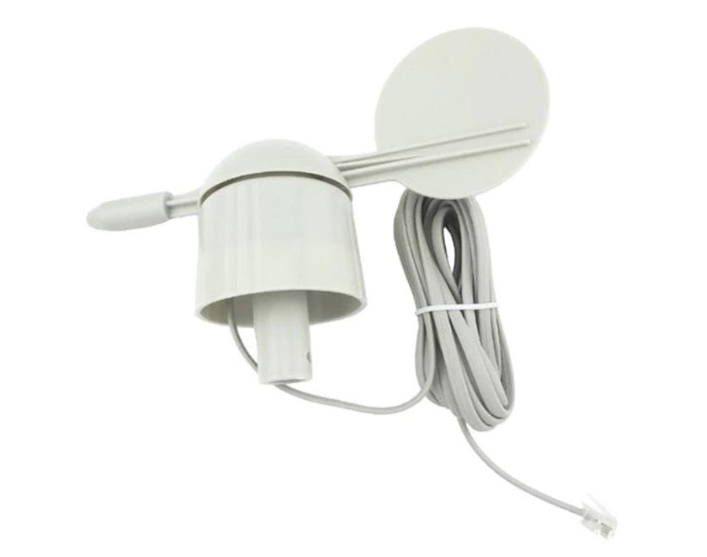
\includegraphics[width=0.5\textwidth]{implementering/vindretning.png}
    \caption{Vindretningssensoren.}
    \label{fig:vindretning}
\end{figure}


\subsubsection{Regn}

Nedbørsmåleren består av to selv-tømmende beholdere, som fylles opp og tipper over etter en gitt mengde nedbør. Når den ene beholderen er fylt opp og tippet over, renner vannet ut under sensoren, og den nye beholderen blir plassert under vanninntaket. Denne sensoren bruker også en reed-kontakt, som trigges av en magnet hver gang en beholder tipper over. Ved å telle antall ganger bryteren lukkes og multiplisere det med mengden nedbør før en beholder tipper, som i databladet er gitt til å være 0,2794 mm, beregnes mengden nedbør som har falt i et gitt tidsrom.

\subsubsection{Kretskort til sensorer}

For enkelt å kunne koble alle sensorene til Raspberry Pi-en, brukes et kretskort som kobler alt sammen. I tillegg til kontakter for enkelt å koble av og på alle sensorene, inneholder kretskortet en analog til digital-omformer, siden en Raspberry Pi ikke inkluderer dette. ADC-en som brukes er en MCP3221A5T fra Microchip. Omformeren tar inn et analogt signal, og kommuniserer direkte over I2C-buss-protokollen med Raspberry Pi-en. Det eneste signalet som trenger en ADC er signalet fra vindretningssensoren. Luftsensoren kommuniserer direkte via I2C-bussen uten en ADC, og anemometeret og nedbørssensoren kobles til hver sin GPIO-pin på Rasperry Pi-en via kretskortet, som sender ut et digitalt signal. Figur x og x under viser henholdsvis kretstegningen og 3D-modell av dette kretskortet.

\begin{figure}[H]
    \centering
    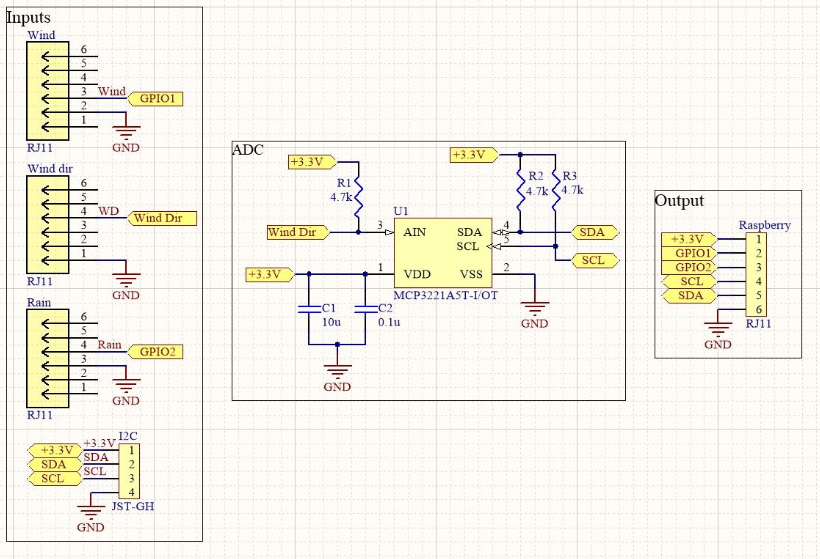
\includegraphics[width=0.8\textwidth]{implementering/sensorkretskort_krets.png}
    \caption{Kretsskjema for kretskortet til sensorene.}
    \label{fig:sensorkretskort_krets}
\end{figure}

\begin{figure}[H]
    \centering
    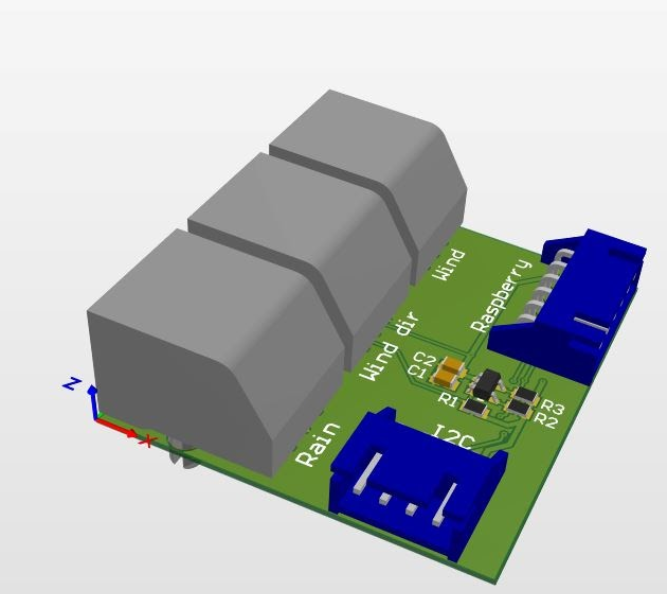
\includegraphics[width=0.5\textwidth]{implementering/sensorkretskort_3d.png}
    \caption{3d-modell av kretskortet til sensorene.}
    \label{fig:sensorkretskort_3d}
\end{figure}


%https://www.argentdata.com/files/80422_datasheet.pdf
%http://ww1.microchip.com/downloads/en/DeviceDoc/20001732E.pdf


\subsection{Nettside}

\todo{Bilde eller figur av nettside}

Nettsiden har som mål å vise informasjonen som hentes inn av både fugletelleren og værstasjonen. Til dette brukes Python-rammeverket Dash \cite{dash}. Dash er laget spesifikt for å vise og prosessere store mengder data i enkle grafer og oppgi disse på en statisk nettside. 

Det kjøres et backend-program som har som oppgave å hente all data fra databasen som er nevnt i \autoref{subsubsec:telemetri}, telemetri. Deretter prosesserer og filtrerer programmet data slik at det ikke bare er punktdata, men data basert på timer, dager, måneder osv. Dette krever kraftige sortering- og filtreringsalgoritmer. Noen av disse algoritmene er allerede implementert, men noen må også implementeres med vanlige funksjoner i Python. 

Store deler av nettsiden fungerer på samme måte. Det kjøres en funksjon om du velger noe data, eller ber nettsiden hente et nytt datasett. Det vil derfor kun gis noen eksempler i avsnittene under, og hele nettsiden kan leses på GitHub\todo{Må legge inn URL og kilde.}

Bilde?\todo{Kanskje et flytdiagram?}

\subsubsection{Rammeverket}

Nettsiden er basert på rammeverket \textbf{Dash} \cite{dash}, som er en kombinasjon og mellomledd mellom nettside-rammeverket for statiske nettsider, \textbf{flask} \cite{flask} og javascript biblioteket \textbf{plotly} \cite{plotly} for å plotte data.

Dash fungerer ved å bruke spesialobjekter fra plotly som ''graph'' og ''slider'', og vanlige \mintinline{html}{html} objekter som \mintinline{html}{div} og \mintinline{html}{header}. Disse defineres i en \mintinline{html}{json} liste, se et enkelt eksempel under i \autoref{code:dashExample1}. 

\begin{code}
\begin{minted}[mathescape,
               linenos,
               numbersep=5pt,
               gobble=2,
               frame=lines,
               framesep=2mm]{python}
    import dash_core_components as dcc

    dcc.Dropdown(
        options=[
            {'label': 'New York City', 'value': 'NYC'},
            {'label': 'Montréal', 'value': 'MTL'},
            {'label': 'San Francisco', 'value': 'SF'}
        ],
        value='MTL'
    )
\end{minted}
\caption{Eksempel på hvordan implementere en ''dropdown'' i dash.}
\label{code:dashExample1}
\end{code}

Det Dash implementerer i flask, er hvordan lage mer interaktive nettsider ved å legge til \textbf{callbacks}, funksjoner som kjører når du f.eks. trykker på en knapp, eller endrer på zoom i en graf.
Det er slik store deler av nettsiden er bygget opp, ved at brukeren endrer på hvilke objekter som er valgt eller drar i en slider. Da vil det skje en ''callback'' som vil kunne endre på data og deretter oppdatere nettsiden. En generell callback som er brukt mye i nettsiden til jolyu er å oppdatere hvilke data som er valgt fra grafen. Et eksempel er i \autoref{code:dashExample2}. Denne tar inn \mintinline{python}{selectedData} fra en graf med id \mintinline{python}{monthAverage} og returnerer data til en lagringssted med id \mintinline{python}{day_selector}. 

\begin{code}
\begin{minted}[mathescape,
               linenos,
               numbersep=5pt,
               gobble=2,
               frame=lines,
               framesep=2mm]{python}
    @app.callback(
        Output("day_selector", "data"), # Det er her retur-funksjonen returnerer ting
        [Input("monthAverage", "selectedData"), # Input fra en graf og en slider
        Input("time_slider", "value")],
    )
    def UpdateDaySel(daySelector, timeSlider):
        days = []
        if daySelector is None:
            days = TimeSliderToDate(timeSlider)
        else:
            days = daySelector["range"]["x"]
        print(days)
        return days
\end{minted}
\caption{Et reelt eksempel på hvordan callbacks brukes på nettsiden. Oppdaterer data fra en graf.}
\label{code:dashExample2}
\end{code}


\subsubsection{Sortering og filtrering}

Sortering og filtrering kan gjøres på veldig mange måter. Det enkleste og ofte det beste er å bruke innebygde funksjoner. På nettsiden brukes en avansert liste, ligner på en SQL-database, som heter \mintinline{python}{dataframe} fra \textbf{pandas} \cite{dataframe}. Den har sine egne sorteringsalgoritmer som brukes aktivt. 

Den mest intense sorteringen er å samle all punktdataen til måneder (eller uker/dager), da det kan være flere hundre tusen punkter i dataen, ønskes det at sorteringen skal være effektiv. Derfor brukes de innebygde funksjonene for akkurat dette formålet. I \autoref{code:dfSortEx1} kan det ses hvordan bare funksjonen \mintinline{python}{dataframe.resample().sum()} brukes for å summere alle punkter i en måned sammen til et enkelt punkt.

\begin{code}
\begin{minted}[mathescape,
               linenos,
               numbersep=5pt,
               gobble=2,
               frame=lines,
               framesep=2mm]{python}
    def DataToMonths(data):
        df = data.resample('M').sum()
        return(df)
    
    def DataToDays(df):
        df = df.resample('D').sum()
        return(df)
\end{minted}
\caption{Funksjoner som sorterer punkter på måneder og dager.}
\label{code:dfSortEx1}
\end{code}

\subsubsection{Database}

\subsection{Strukturelt}

Stativet boksen og værstasjonen skal festes til er vist i figur \ref{fig:Stativ}. Her vil boksen festes til stangen ca ?? m over bakken mens øverst ?? m over bakken er modulene til værstasjonen festet. 

\begin{figure}[H]
    \centering
    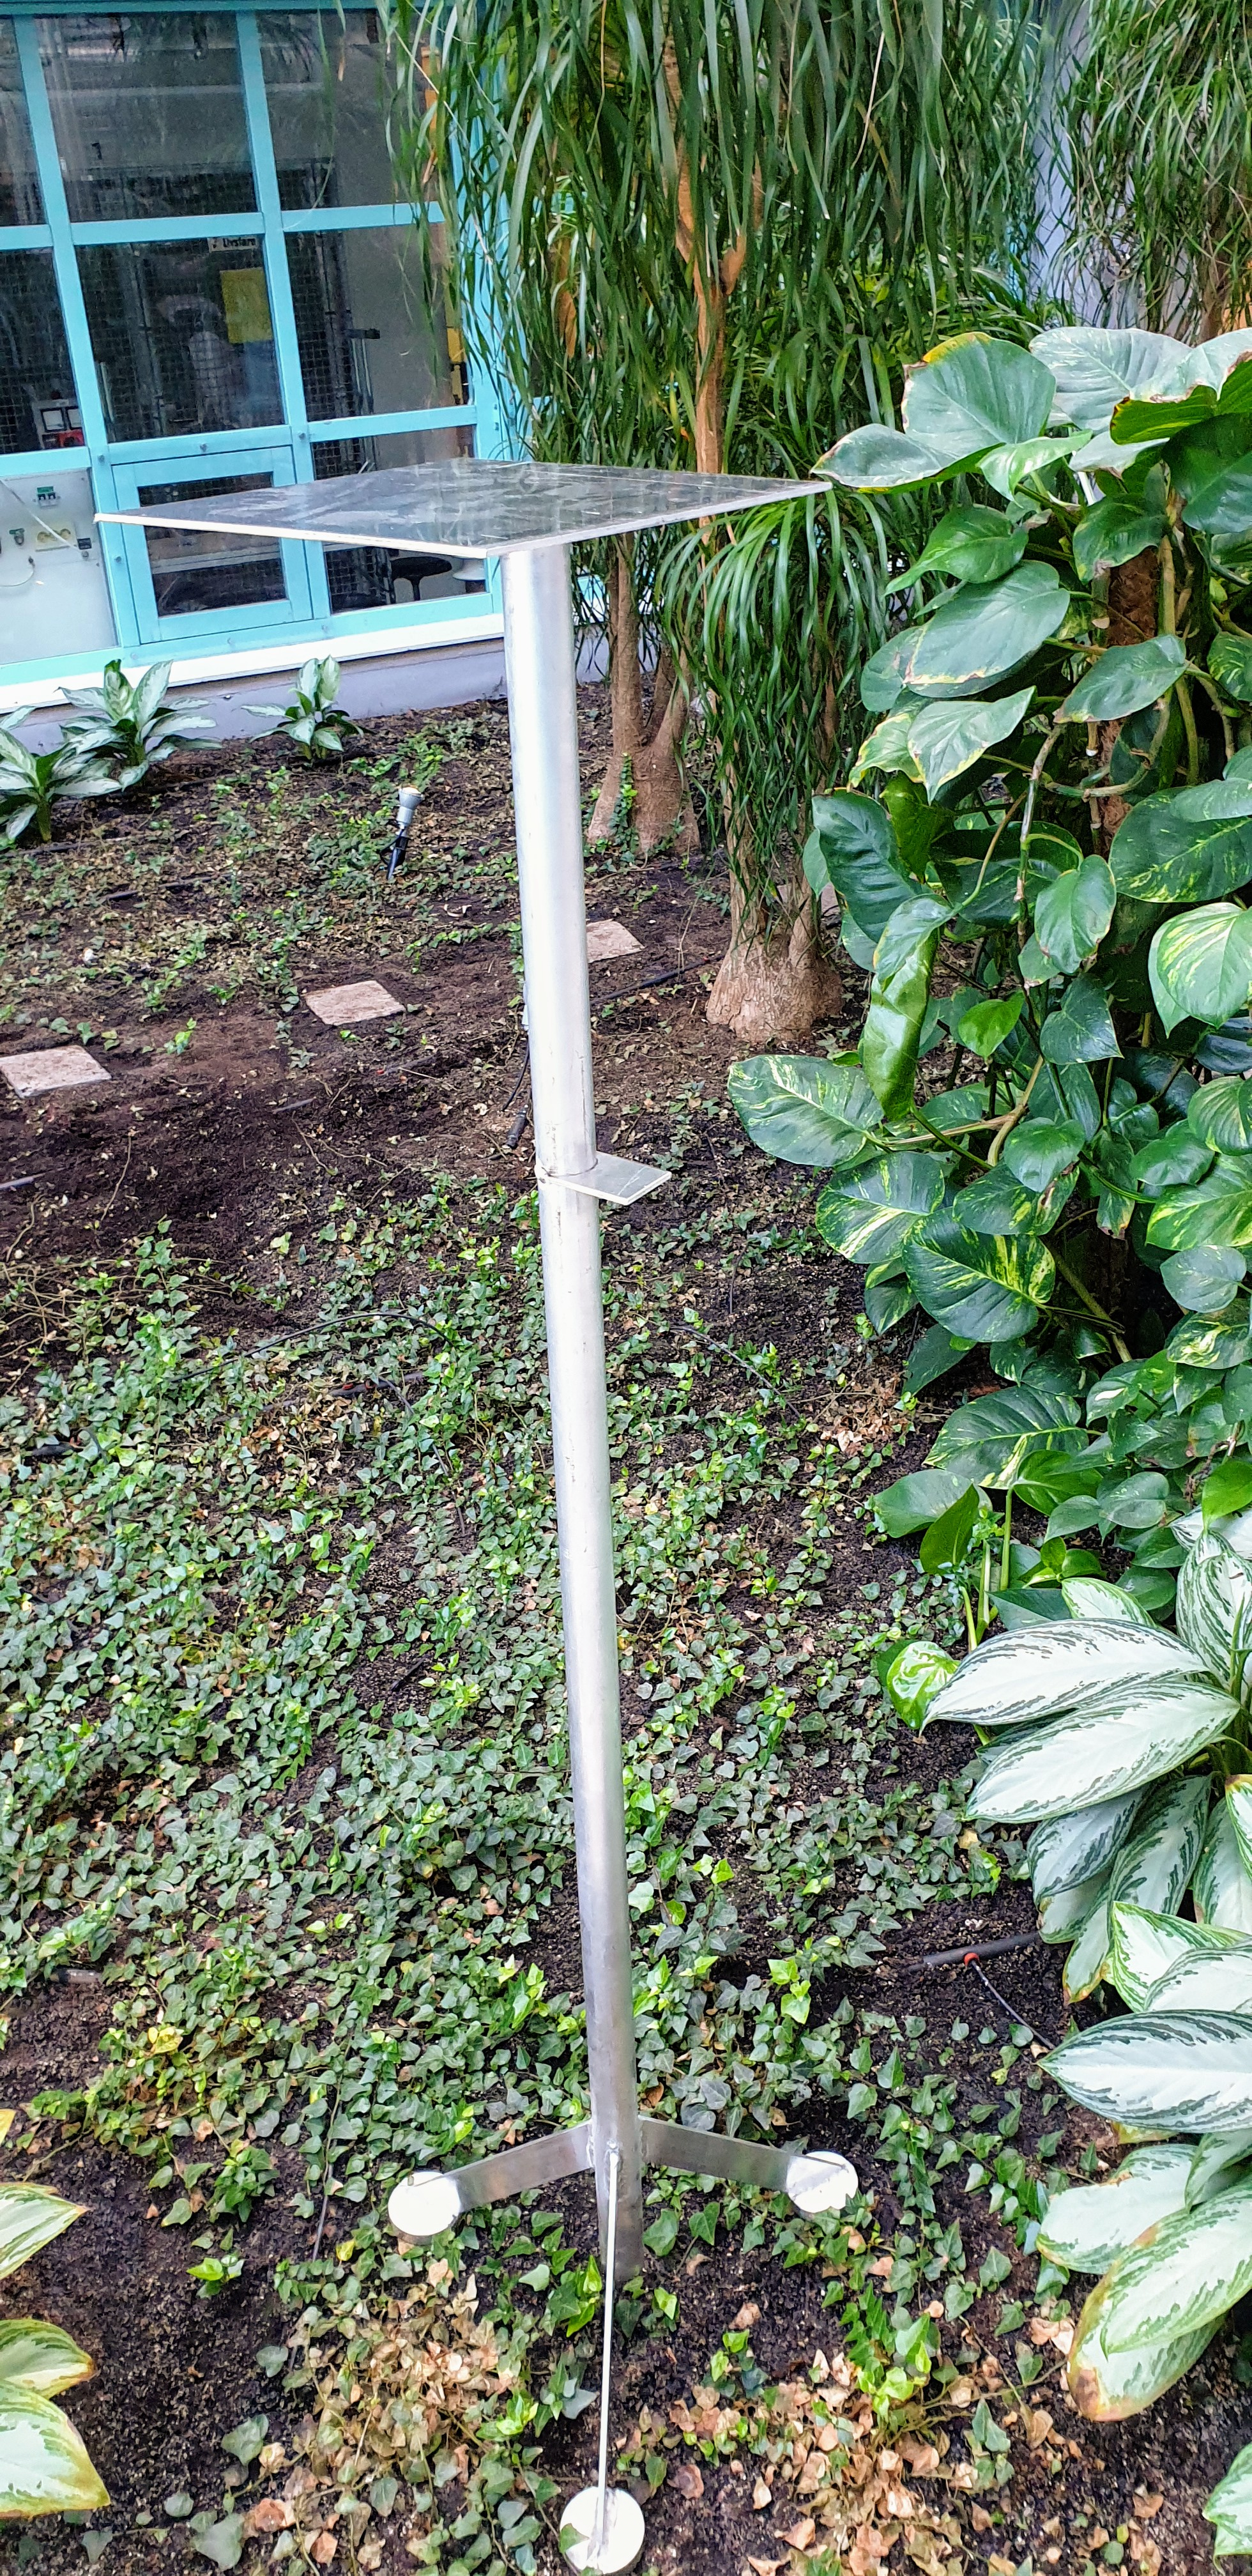
\includegraphics[width=.7\textwidth]{implementering/Stativ.jpg}
    \caption{Stativ for boks og værstasjon.\todo{Sett inn bilde}}
    \label{fig:Stativ}
\end{figure}

En 3D-modell av boksen er vist i figur \ref{fig:boks}.
\begin{figure}[H]
    \centering
    \includegraphics[width=.7\textwidth]{}
    \caption{En 3D modell av boksen som skal holde kamera og prosesseringsenheten.}
    \label{fig:boks}
\end{figure}
